\documentclass[11pt]{article}
\usepackage[utf8]{inputenc}
\usepackage[english]{babel}
\usepackage{pdfpages}
\usepackage{hyperref}
\usepackage{float}
\usepackage{verbatim}
\usepackage{graphicx}

\title{Network}
\author{Riccardo Scheda}

\begin{document}

\maketitle

\section{Modello}
All'inizio considero un network (diretto) di 5 geni in questa forma:
\begin{figure}[ht!]
  \center
  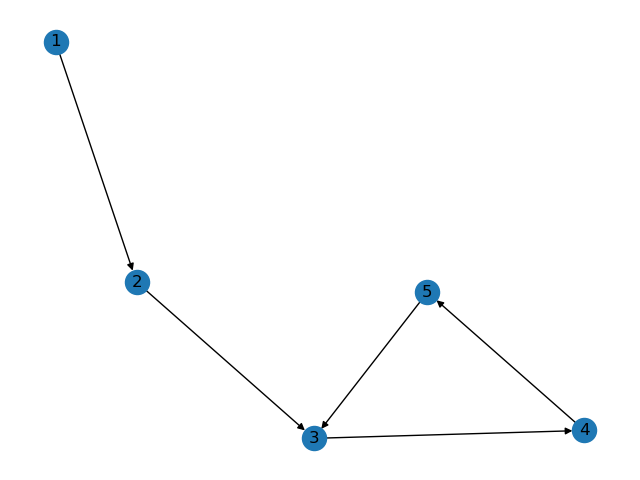
\includegraphics[scale=0.5]{network.png}
  \label{fig:net}
\end{figure}
Dove i nodi possono assumere i valori 0 o 1.
Quindi la matrice di adiacenza A sarà:
$$
\bold{A} = \left (
\begin{array}{ccccc}

0 & 0 & 0 & 0 & 0  \\
1 & 0 & 0 & 0 & 0  \\
0 & 1 & 0 & 0 & 1  \\
0 & 0 & 1 & 0 & 0  \\
0 & 0 & 0 & 1 & 0  \\

\end{array}
\right )
$$

Successivamente per evolvere il sistema considero il network come un vettore e applico A al vettore, (In realtà non è proprio un prodotto matrice-vettore ma è un prodotto riga per colonna in cui poi sostituisco il risultato con 1 se l'elemento di matrice è diverso da zero.)
Quindi ad esempio se ho una condizione iniziale del tipo:
$$
\textbf{n}_0 = \left ( 
\begin{array}{c}
1 \\
0 \\
0 \\
0 \\
0 \\
\end{array}
\right ) 
$$

avremo $n_1$:
$$
\textbf{n}_1= A \textbf{n}_0 = \left ( 
\begin{array}{c}
0 \\
1 \\
0 \\
0 \\
0 \\
\end{array}
\right ) 
$$

Quindi in generale abbiamo 
$$
\textbf{n}_{n+1}= A \textbf{n}_n = A^n \textbf{n}_0
$$

Con questo network arriviamo allo stato stazionario in cui ciclicamente si attivano i nodi 3,4 e 5.

Infatti se consideriamo il network come una sequenza di 1 e 0: $n_0 = 10000$ ad ogni step possiamo costruire il network delle configurazioni della stringa, dove i link
sono dati dal passaggio da una stringa ad un'altra step per step:
\begin{figure}[ht!]
  \center
  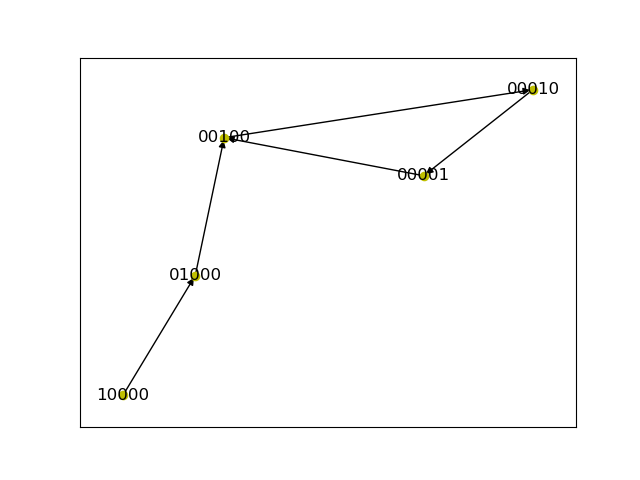
\includegraphics[scale=0.5]{confi.png}
  \label{fig:net}
\end{figure}


\section{Aggiunta del nodo ambiente}
Se al network aggiungiamo un sesto nodo che rappresenta l'ambiente, e se lo attiviamo dopo un certo tempo t, mantenendolo sempre attivo,  il sistema collassa ad uno stato limite in cui i noid 3, 4 e 5 rimangono sempre attivi.

in questo caso il network diventa:
\begin{figure}[ht!]
  \center
  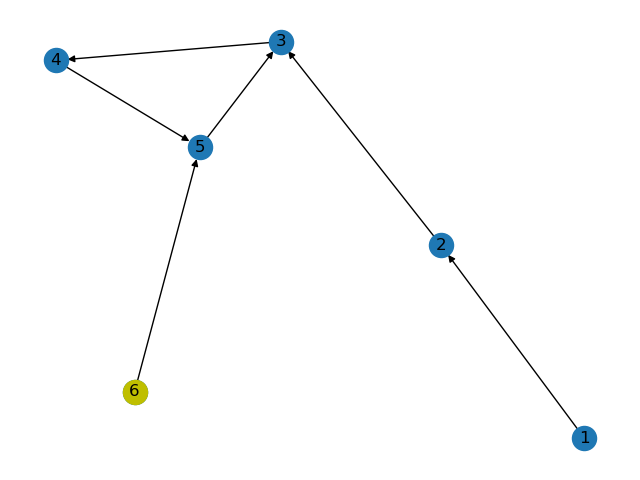
\includegraphics[scale=0.5]{env.png}
  \label{fig:net}
\end{figure}

A questo punto il network delle configurazioni cambia, e considerando tutte le possibili condizioni iniziali (in cui il nodo i-esimo è attivo e gli altri no) il sistema collassa sempre alla stessa configurazione 001111:

\begin{figure}[ht!]
  \center
  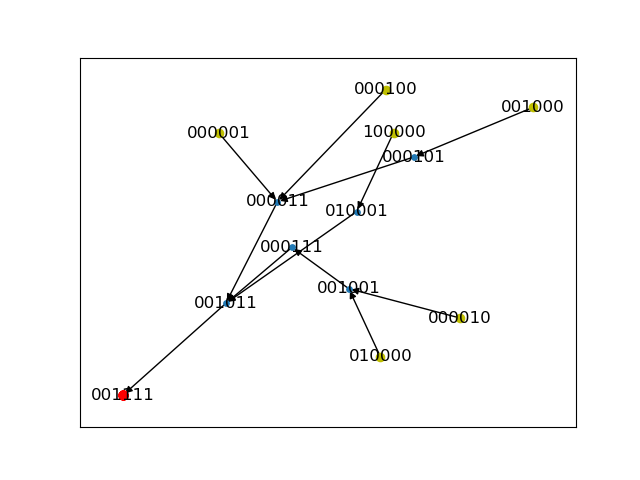
\includegraphics[scale=0.5]{confenv.png}
  \label{fig:net}
\end{figure}


\end{document}
